% Options for packages loaded elsewhere
\PassOptionsToPackage{unicode}{hyperref}
\PassOptionsToPackage{hyphens}{url}
\PassOptionsToPackage{dvipsnames,svgnames,x11names}{xcolor}
%
\documentclass[
  authoryear,
  preprint,
  1p]{elsarticle}

\usepackage{amsmath,amssymb}
\usepackage{iftex}
\ifPDFTeX
  \usepackage[T1]{fontenc}
  \usepackage[utf8]{inputenc}
  \usepackage{textcomp} % provide euro and other symbols
\else % if luatex or xetex
  \usepackage{unicode-math}
  \defaultfontfeatures{Scale=MatchLowercase}
  \defaultfontfeatures[\rmfamily]{Ligatures=TeX,Scale=1}
\fi
\usepackage{lmodern}
\ifPDFTeX\else  
    % xetex/luatex font selection
\fi
% Use upquote if available, for straight quotes in verbatim environments
\IfFileExists{upquote.sty}{\usepackage{upquote}}{}
\IfFileExists{microtype.sty}{% use microtype if available
  \usepackage[]{microtype}
  \UseMicrotypeSet[protrusion]{basicmath} % disable protrusion for tt fonts
}{}
\makeatletter
\@ifundefined{KOMAClassName}{% if non-KOMA class
  \IfFileExists{parskip.sty}{%
    \usepackage{parskip}
  }{% else
    \setlength{\parindent}{0pt}
    \setlength{\parskip}{6pt plus 2pt minus 1pt}}
}{% if KOMA class
  \KOMAoptions{parskip=half}}
\makeatother
\usepackage{xcolor}
\setlength{\emergencystretch}{3em} % prevent overfull lines
\setcounter{secnumdepth}{5}
% Make \paragraph and \subparagraph free-standing
\makeatletter
\ifx\paragraph\undefined\else
  \let\oldparagraph\paragraph
  \renewcommand{\paragraph}{
    \@ifstar
      \xxxParagraphStar
      \xxxParagraphNoStar
  }
  \newcommand{\xxxParagraphStar}[1]{\oldparagraph*{#1}\mbox{}}
  \newcommand{\xxxParagraphNoStar}[1]{\oldparagraph{#1}\mbox{}}
\fi
\ifx\subparagraph\undefined\else
  \let\oldsubparagraph\subparagraph
  \renewcommand{\subparagraph}{
    \@ifstar
      \xxxSubParagraphStar
      \xxxSubParagraphNoStar
  }
  \newcommand{\xxxSubParagraphStar}[1]{\oldsubparagraph*{#1}\mbox{}}
  \newcommand{\xxxSubParagraphNoStar}[1]{\oldsubparagraph{#1}\mbox{}}
\fi
\makeatother


\providecommand{\tightlist}{%
  \setlength{\itemsep}{0pt}\setlength{\parskip}{0pt}}\usepackage{longtable,booktabs,array}
\usepackage{calc} % for calculating minipage widths
% Correct order of tables after \paragraph or \subparagraph
\usepackage{etoolbox}
\makeatletter
\patchcmd\longtable{\par}{\if@noskipsec\mbox{}\fi\par}{}{}
\makeatother
% Allow footnotes in longtable head/foot
\IfFileExists{footnotehyper.sty}{\usepackage{footnotehyper}}{\usepackage{footnote}}
\makesavenoteenv{longtable}
\usepackage{graphicx}
\makeatletter
\def\maxwidth{\ifdim\Gin@nat@width>\linewidth\linewidth\else\Gin@nat@width\fi}
\def\maxheight{\ifdim\Gin@nat@height>\textheight\textheight\else\Gin@nat@height\fi}
\makeatother
% Scale images if necessary, so that they will not overflow the page
% margins by default, and it is still possible to overwrite the defaults
% using explicit options in \includegraphics[width, height, ...]{}
\setkeys{Gin}{width=\maxwidth,height=\maxheight,keepaspectratio}
% Set default figure placement to htbp
\makeatletter
\def\fps@figure{htbp}
\makeatother

\makeatletter
\@ifpackageloaded{caption}{}{\usepackage{caption}}
\AtBeginDocument{%
\ifdefined\contentsname
  \renewcommand*\contentsname{Table of contents}
\else
  \newcommand\contentsname{Table of contents}
\fi
\ifdefined\listfigurename
  \renewcommand*\listfigurename{List of Figures}
\else
  \newcommand\listfigurename{List of Figures}
\fi
\ifdefined\listtablename
  \renewcommand*\listtablename{List of Tables}
\else
  \newcommand\listtablename{List of Tables}
\fi
\ifdefined\figurename
  \renewcommand*\figurename{Figure}
\else
  \newcommand\figurename{Figure}
\fi
\ifdefined\tablename
  \renewcommand*\tablename{Table}
\else
  \newcommand\tablename{Table}
\fi
}
\@ifpackageloaded{float}{}{\usepackage{float}}
\floatstyle{ruled}
\@ifundefined{c@chapter}{\newfloat{codelisting}{h}{lop}}{\newfloat{codelisting}{h}{lop}[chapter]}
\floatname{codelisting}{Listing}
\newcommand*\listoflistings{\listof{codelisting}{List of Listings}}
\makeatother
\makeatletter
\makeatother
\makeatletter
\@ifpackageloaded{caption}{}{\usepackage{caption}}
\@ifpackageloaded{subcaption}{}{\usepackage{subcaption}}
\makeatother
\journal{Psychometrika}

\ifLuaTeX
  \usepackage{selnolig}  % disable illegal ligatures
\fi
\usepackage[]{natbib}
\bibliographystyle{elsarticle-harv}
\usepackage{bookmark}

\IfFileExists{xurl.sty}{\usepackage{xurl}}{} % add URL line breaks if available
\urlstyle{same} % disable monospaced font for URLs
\hypersetup{
  pdftitle={Causes and effects in Dichotomous Comparative Judgments: an information-theoretical system of plausible mechanism},
  pdfauthor={Jose Manuel Rivera Espejo; Tine van van Daal; Sven De De Maeyer; Steven Gillis},
  pdfkeywords={causal inference, probability, Thurstone, comparative
judgement, directed acyclic graph, structural causal models, statistical
modeling},
  colorlinks=true,
  linkcolor={blue},
  filecolor={Maroon},
  citecolor={Blue},
  urlcolor={Blue},
  pdfcreator={LaTeX via pandoc}}


\setlength{\parindent}{6pt}
\begin{document}

\begin{frontmatter}
\title{Causes and effects in Dichotomous Comparative Judgments: an
information-theoretical system of plausible mechanism}
\author[1]{Jose Manuel Rivera Espejo%
\corref{cor1}%
}
 \ead{JoseManuel.RiveraEspejo@uantwerpen.be} 
\author[1]{Tine van Daal%
%
}
 \ead{tine.vandaal@uantwerpen.be} 
\author[1]{Sven De Maeyer%
%
}
 \ead{sven.demaeyer@uantwerpen.be} 
\author[2]{Steven Gillis%
%
}
 \ead{steven.gillis@uantwerpen.be} 

\affiliation[1]{organization={University of Antwerp, Training and
education sciences},,postcodesep={}}
\affiliation[2]{organization={University of
Antwerp, Linguistics},,postcodesep={}}

\cortext[cor1]{Corresponding author}




        
\begin{abstract}
Dichotomous Comparative Judgment (DCJ) requires judges to compare pairs
of stimuli to determine which one exhibits a higher degree of a specific
trait. DCJ has proven effective and reliable across various fields
\citep{Pollitt_2012b, Jones_2015, vanDaal_et_al_2016, Bartholomew_et_al_2018, Lesterhuis_2018, Bartholomew_et_al_2020, Marshall_et_al_2020, Boonen_et_al_2020}.
However, despite the method's widespread use, existing literature lacks
a clear explanation of the complexities and assumptions underpinning the
DCJ system, as well as the plausible mechanisms through which DCJ data
could be generated. This study addresses these issues by representing
DCJ within the framework of causal inference. Specifically, utilizing
the structural approach, the study develops a scientific model to
clarify plausible causal assumptions and mechanisms inherent in the DCJ
system. The study then translates this model into a probabilistic
statistical model to estimate statistical relationships and infer causal
effects within the system. This research provides a robust probabilistic
foundation for the statistical analysis of DCJ data, building upon
Thurstone's law of comparative judgment \citeyearpar{Thurstone_1927}.
Its findings offer valuable insights for researchers and analysts
designing and implementing DCJ experiments.
\end{abstract}





\begin{keyword}
    causal inference \sep probability \sep Thurstone \sep comparative
judgement \sep directed acyclic graph \sep structural causal
models \sep 
    statistical modeling
\end{keyword}
\end{frontmatter}
    

\section{Introduction}\label{sec-introduction}

In contemporary contexts, Thurstone's law of comparative judgment
\citeyearpar{Thurstone_1927} primarily refers to the method of
\emph{dichotomous} comparative judgment
\citep[DCJ,][]{Pollitt_2012a, Pollitt_2012b}. In DCJ, a judge assesses
the relative manifestation of a \emph{trait} within a pair of stimuli.
This assessment results in a dichotomous value indicating which stimulus
possesses a higher degree of the trait. After different judges perform
multiple rounds of pairwise comparisons, an outcome vector is produced.
This vector is modeled using the Bradley-Terry-Luce model
\citep[BTL,][]{Bradley_et_al_1952, Luce_1959}, which creates a score
that corresponds with the trait of interest. This score is then used to
rank the stimuli from lowest to highest or to evaluate the influence of
certain variables on the stimuli's positions in the ranking.

DCJ has proven effective in assessing competencies and traits
predominantly within the educational realm, as demonstrated by
\citet{Pollitt_2012b}, \citet{Jones_2015}, \citet{vanDaal_et_al_2016},
\citet{Bartholomew_et_al_2018}, \citet{Lesterhuis_2018},
\citet{Bartholomew_et_al_2020}, and \citet{Marshall_et_al_2020}.
However, its application transcends education, as exemplified by
\citet{Boonen_et_al_2020}. The methodology has also evolved to include
multiple, as opposed to pairwise comparisons
\citep{Luce_1959, Placket_1975}, and to accommodate comparisons with
ordinal outcomes \citep{Tutz_1986, Agresti_1992}. Overall, research
suggests that DCJ offers an alternative and efficient approach to
measurement and evaluation, characterized by its reliability and
validity
\citep{Lesterhuis_2018, vanDaal_2020, Marshall_et_al_2020, Bouwer_et_al_2023}.
Nevertheless, despite the method's widespread use, existing literature
lacks a clear representation of the plausible mechanisms through which
DCJ data could be generated. Particularly, there is no depiction of the
complexity and the assumptions underpinning the DCJ system, nor how
different assessment factors can potentially influence the observed DCJ
outcome.

According to \citet{Verhavert_et_al_2019} and \citet{vanDaal_2020},
several assessment factors interact and influence the method's outcome.
These factors include the number and characteristics of the stimuli,
their \emph{proximity} in terms of the assessed trait, the number of
comparison per stimulus, and the pairing algorithm used. Furthermore,
since the method relies on judges' assessments, the number and
characteristics of judges, their \emph{discrimination} abilities, and
the number of comparisons per judge also play pivotal roles. Moreover,
when the stimuli represent sub-units of higher-levels units, factors
such as the number and characteristics of these units, along with their
\emph{proximity} in terms of the assessed trait, can significantly
influence the outcome. For example, in \citet{vanDaal_et_al_2016}, the
authors assessed the academic writing skills of university students
(units) using multiple argumentative essays (sub-units).

Although several studies have examined the individual impact of these
factors on the method's reliability
\citep{Bramley_2015, Pollitt_2012b, Bramley_et_al_2019, Verhavert_et_al_2019, Crompvoets_et_al_2022, vanDaal_et_al_2017, Gijsen_et_al_2021, Bouwer_et_al_2023},
none, to the best of the authors' knowledge, have provided a transparent
depiction of the DCJ system and the mechanisms generating the DCJ
outcome. This study aims to fill this gap by representing DCJ within the
framework of causal inference. Specifically, utilizing the structural
approach to causal inference, the study develops a scientific model to
clarify plausible causal assumptions and mechanisms inherent in the DCJ
system. The study then translates the scientific model into a
probabilistic statistical model. This model aims to produce statistical
estimates to draw inferences about plausible causal relationships within
the DCJ system.

Ultimately, this study provides a robust causal and probabilistic
foundation for the statistical analysis of DCJ data, building upon
Thurstone's law of comparative judgment \citeyearpar{Thurstone_1927}.
Consequently, its findings offer valuable insights for researchers and
analysts designing and implementing DCJ experiments.

\section{Theoretical framework}\label{sec-framework}

This section introduces fundamental concepts in causal inference but
does not offer a comprehensive description of causal inference methods.
Readers interested in deeper exploration should consult introductory
papers like \citet{Pearl_2010}, \citet{Rohrer_2018}, \citet{Pearl_2019},
and \citet{Cinelli_et_al_2020}. They may also find introductory books
such as \citet{Pearl_et_al_2018}, \citet{Neal_2020} and
\citet{McElreath_2020} useful. For more advanced study, seminal
intermediate papers like \citet{Neyman_et_al_1923}, \citet{Rubin_1974},
\citet{Spirtes_et_al_1991}, and \citet{Sekhon_2009}, as well as books
like \citet{Pearl_2009}, \citet{Morgan_et_al_2014} and
\citet{Hernan_et_al_2020} are recommended.

\subsection{The structural approach to causal
inference}\label{sec-framework-structural}

Empirical research addresses real-world challenges by relying on
evidence gathered through observation and experimentation. In this
context, researchers typically frame their research questions as
\emph{estimands} or \emph{targets of inference}. These estimands
represent the specific quantities the study aims to determine
\citep{Everitt_et_al_2010}. For instance, a study might examine the
question, ``To what extent do different teaching methods (\(T\))
influence students' conceptual understanding of a topic (\(Y\))?'' To
investigate this, the study could randomly assign students to two
groups, each using a different teaching method \((T_{i}=\{1,2\})\).
Students' conceptual understanding of the topic could be evaluated
through pairwise comparisons, resulting in a dichotomous outcome
\((Y_{i}=\{0,1\})\), indicating which student among those compared has a
higher level of understanding. The research question could be then
framed as the estimand, ``\emph{On average}, is there a difference in
conceptual understanding of the topic between the two groups of
students?'' This estimand could be mathematically expressed by the
associational quantity \(E[Y_{i}| T_{i}=1] - E[Y_{i}| T_{i}=2]\), where
\(E[\cdot]\) denotes the expected value. An example of this approach is
seen in \citet{Jones_et_al_2019}.

Researchers then proceed to identify the estimands.
\emph{Identification} refers to the process of accurately computing an
estimand using an estimator. An \emph{estimator} is a method or function
that maps data into an estimate \citep{Neal_2020}. \emph{Estimates} are
numerical values that approximate the estimand and are derived through
\emph{estimation}, which refer to the process of integrating data with
an estimator \citep{Everitt_et_al_2010}. Although various methods can
approximate an estimand, researchers prioritize estimators with
desirable properties that ensure the accuracy of estimates. For
instance, the BTL model \citep{Bradley_et_al_1952, Luce_1959} is an
estimator known for its effectiveness in modeling pairwise comparisons,
yielding accurate estimates for the target of inference discussed
earlier, as long as the assumptions of the model are met.

However, many studies aim to understand the mechanisms underlying
specific data types and also seek to establish causal relationships
rather than merely infer associations. In the earlier example, the
differences between groups obtained using the BTL model, referred to as
the associational estimates, can be interpreted as causal because the
data were collected through a randomized experiment. Randomized
experiments enable the causal interpretation of associational estimates
by ensuring several key properties, including common support, no
interference, and consistency \citep{Morgan_et_al_2014, Neal_2020}. The
most crucial property, however, is that randomization effectively
eliminates confounding. \emph{Confounding} occurs when an external
variable influences both the outcome and the variable of interest,
leading to spurious associations \citep{Everitt_et_al_2010}.
Randomization mitigates this issue by decoupling the intervention
assignment mechanism, such as assigning students to different groups,
from other variables and outcomes \citep{Morgan_et_al_2014, Neal_2020}.

Experiments are widely regarded as the gold standard in evidence-based
science \citep{Hariton_et_al_2018, Hansson_2014}, however, researchers
often encounter constraints that limit their ability to conduct
experimental studies. These constraints include ethical concerns, such
as the assignment of individuals to potentially harmful interventions,
and practical limitations, such as the infeasibility of, for example,
assigning individuals to genetic modifications or physical impairments
\citep{Neal_2020}. In these instances, causal inference offers a
valuable alternative for generating causal estimates. \emph{Causal
inference} is a framework designed to identify the causes of phenomena
and estimate their effects using data
\citep{Shaughnessy_et_al_2010, Neal_2020}. Unlike classical statistical
modeling, which focuses primarily on summarizing data and inferring
associations, causal inference provides a rigorous mathematical
framework for analyzing causes and counterfactuals \citep{Pearl_2009}.
Consequently, the framework offers significant theoretical insights that
enhance the design of observational and experimental studies
\citep{McElreath_2020}.

While a detailed explanation of causes and counterfactuals is beyond the
scope of this document, it is important to note that causal inference
addresses the \emph{fundamental problem of causality} through the use of
counterfactuals \citep{Neal_2020}. The framework defines
\emph{individual causal effects} (ICE) as the difference between an
individual's observed and unobserved potential outcomes. These
unobserved potential outcomes, known as \emph{counterfactuals},
represent hypothetical scenarios that are \emph{contrary to fact}, where
alternative outcomes for an individual, resulting from a specific cause,
are neither observed nor observable
\citep{Neal_2020, Counterfactual_2024}. The framework then extends this
estimand to \emph{average causal effects} (ACE), which captures the
difference between sample averages of observed potential outcomes and
counterfactuals. Finally, much like in an experiment, the framework
identifies the ACE from associational estimates by conditioning for a
\emph{sufficient adjustment set} of variables, ensuring the absence of
confounding \citep{Morgan_et_al_2014}.

Several approaches to causal inference and counterfactuals exist, but
two are particularly prominent: the potential outcomes approach, also
known as the Neyman-Rubin causal model
\citep{Neyman_et_al_1923, Rubin_1974}, and the structural approach
\citep{Pearl_2009, Pearl_et_al_2016}. Both approaches employ rigorous
mathematical notation to characterize the ACE, but they do so in
different ways \citep{Neal_2020}. The potential outcomes approach relies
on counterfactual notation, whereas the structural approach employs
do-calculus \citep{Pearl_2009}. Despite these differences, both
notations can be expressed in terms of the other, and both approaches
provide methods for using experimental and observational data to
estimate causal effects \citep{Pearl_2010}.

The structural approach, however, offers a notable advantage over the
potential outcomes approach by allowing the graphical and formal
representation of theories through directed acyclic graphs
\citep[DAG,][]{Pearl_2009, Pearl_et_al_2016, Gross_et_al_2018, Neal_2020}.
DAGs function as heuristics, effectively conveying the presumed causal
structure of a system, referred to as a \emph{scientific model}. They do
not represent detailed statistical models but allow researchers to
deduce which statistical models can provide valid causal inferences,
assuming the causal structure depicted in the DAGs are accurate
\citep{McElreath_2020}. The Identification-Estimation flowchart in
Figure~\ref{fig-IEflow} visually represents this process of
transitioning from estimands to estimates, as well as the application of
the scientific model and data to identify and estimate causal effects.

\begin{figure}

\centering{

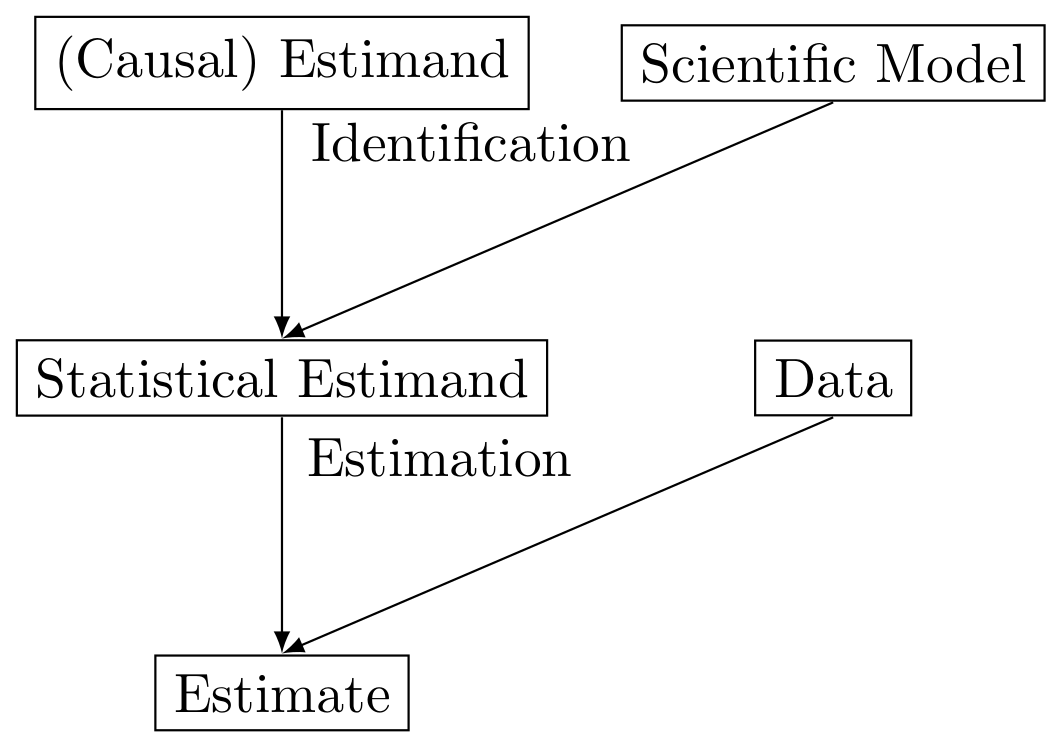
\includegraphics[width=0.4\textwidth,height=\textheight]{images/figures/IEflow.png}

}

\caption{\label{fig-IEflow}Identification-Estimation flowchart.
Extracted and slightly modified from \citet[32]{Neal_2020}}

\end{figure}%

\subsection{DAGs and SCMs}\label{sec-framework-dag}

Graph theory is a branch of mathematics focused on the study of graphs.
Graphs are mathematical structures modeling pairwise relations between
objects. They can represent physical relations, such as electrical
circuits and roadways, and less tangible structures, such as ecosystems
and sociological relations. Graphs have proven useful in various fields,
including computer science, operations research, and the natural and
social sciences \citep{Gross_et_al_2018}.

In statistics, one application incorporating concepts from graph theory
is causal inference. Specifically, the structural approach to causal
inference uses directed acyclic graphs (DAG) to provide a graphical and
formal representation of the causal structure of a system
\citep{Neal_2020}. In this context, a \emph{graph} denotes a collection
of nodes connected by edges, where nodes represent random variables. The
term \emph{directed} indicates the edges of the graph extend from one
node to another, with arrows showing the direction of causal influence.
Moreover, the term \emph{acyclic} indicates the causal influences do not
form a loop, meaning the influences do not cycle back on themselves
\citep{McElreath_2020}.

DAGs offer two key advantages for modeling causal structures. Firstly,
they represent causal relations in a nonparametric and fully interactive
manner. This feature allows for feasible causal analysis strategies
without needing the specification of the type of data or the nature of
the functional dependence among variables \citep{Morgan_et_al_2014}.
Secondly, regardless of complexity, DAGs can represent various causal
structures using only five fundamental building blocks
\citep{Neal_2020, McElreath_2020}. This feature enables the
decomposition of complex structures into basic building blocks,
facilitating the analysis of these structures by focusing on the causal
assumptions associated with each building block individually
\citep{McElreath_2020}. These building blocks can be represented in
three ways: the magnified representation, the standard representation,
and the structural causal model form \citep[SCM,][]{Morgan_et_al_2014}.

\newcommand{\dsep}{\perp\!\!\!\perp}
\newcommand{\ndsep}{\not\!\perp\!\!\!\perp}

\begin{figure}

\begin{minipage}{0.33\linewidth}

\centering{

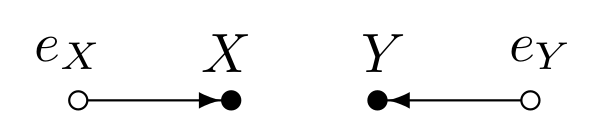
\includegraphics[width=0.8\textwidth,height=\textheight]{images/figures/mdag_bb1.png}

}

\subcaption{\label{fig-mdag_bb1}Two unconnected nodes}

\end{minipage}%
%
\begin{minipage}{0.33\linewidth}

\centering{

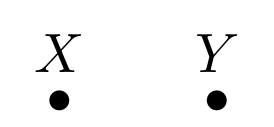
\includegraphics[width=0.35\textwidth,height=\textheight]{images/figures/sdag_bb1.png}

}

\subcaption{\label{fig-sdag_bb1}Two unconnected nodes}

\end{minipage}%
%
\begin{minipage}{0.33\linewidth}

\centering{

\[
\begin{aligned}
  X & := f_{X}(e_{X}) \\
  Y & := f_{Y}(e_{Y}) \\
  e_{X} & \perp\!\!\!\perp e_{Y}
\end{aligned}
\]

}

\subcaption{\label{fig-scm_bb1}Two unconnected nodes}

\end{minipage}%
\newline
\begin{minipage}{0.33\linewidth}

\centering{

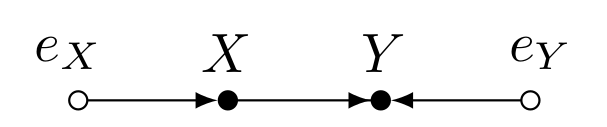
\includegraphics[width=0.8\textwidth,height=\textheight]{images/figures/mdag_bb2.png}

}

\subcaption{\label{fig-mdag_bb2}Two connected nodes or descendant}

\end{minipage}%
%
\begin{minipage}{0.33\linewidth}

\centering{

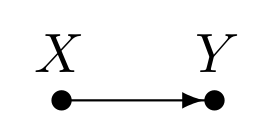
\includegraphics[width=0.35\textwidth,height=\textheight]{images/figures/sdag_bb2.png}

}

\subcaption{\label{fig-sdag_bb2}Two connected nodes or descendant}

\end{minipage}%
%
\begin{minipage}{0.33\linewidth}

\centering{

\[
\begin{aligned}
  X & := f_{X}(e_{X}) \\
  Y & := f_{Y}(X,e_{Y}) \\
  e_{X} & \perp\!\!\!\perp e_{Y}
\end{aligned}
\]

}

\subcaption{\label{fig-scm_bb2}Two connected nodes or descendant}

\end{minipage}%
\newline
\begin{minipage}{0.33\linewidth}

\centering{

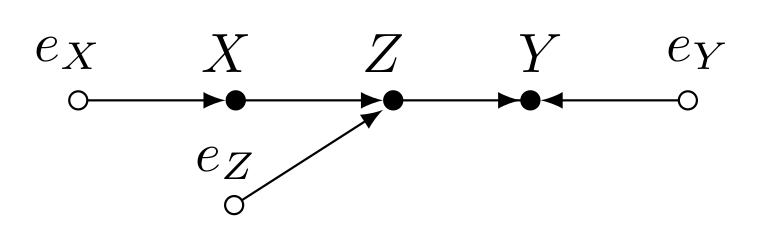
\includegraphics[width=1\textwidth,height=\textheight]{images/figures/mdag_bb3.png}

}

\subcaption{\label{fig-mdag_bb3}Chain or pipe}

\end{minipage}%
%
\begin{minipage}{0.33\linewidth}

\centering{

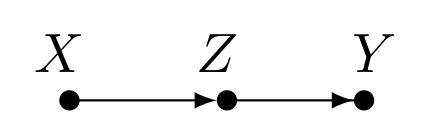
\includegraphics[width=0.55\textwidth,height=\textheight]{images/figures/sdag_bb3.png}

}

\subcaption{\label{fig-sdag_bb3}Chain or pipe}

\end{minipage}%
%
\begin{minipage}{0.33\linewidth}

\centering{

\[
\begin{aligned}
  X & := f_{X}(e_{X}) \\
  Z & := f_{Z}(X,e_{Z}) \\
  Y & := f_{Y}(Z,e_{Y}) \\
  e_{X} & \perp\!\!\!\perp e_{Y} \\
  e_{X} & \perp\!\!\!\perp e_{Z} \\
  e_{Z} & \perp\!\!\!\perp e_{Y}
\end{aligned}
\]

}

\subcaption{\label{fig-scm_bb3}Chain or pipe}

\end{minipage}%
\newline
\begin{minipage}{0.33\linewidth}

\centering{

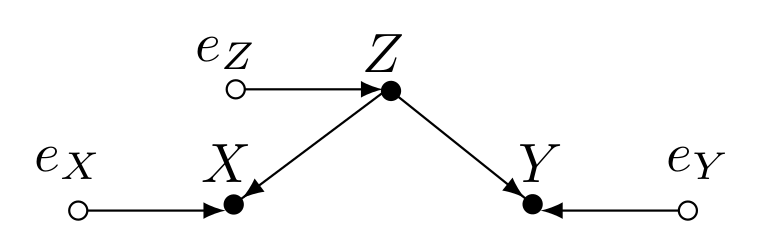
\includegraphics[width=1\textwidth,height=\textheight]{images/figures/mdag_bb4.png}

}

\subcaption{\label{fig-mdag_bb4}Fork}

\end{minipage}%
%
\begin{minipage}{0.33\linewidth}

\centering{

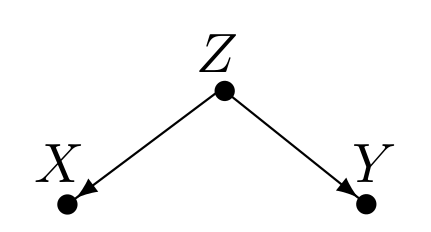
\includegraphics[width=0.55\textwidth,height=\textheight]{images/figures/sdag_bb4.png}

}

\subcaption{\label{fig-sdag_bb4}Fork}

\end{minipage}%
%
\begin{minipage}{0.33\linewidth}

\centering{

\[
\begin{aligned}
  X & := f_{X}(Z,e_{X}) \\
  Z & := f_{Z}(e_{Z}) \\
  Y & := f_{Y}(Z,e_{Y}) \\
  e_{X} & \perp\!\!\!\perp e_{Y} \\
  e_{X} & \perp\!\!\!\perp e_{Z} \\
  e_{Z} & \perp\!\!\!\perp e_{Y}
\end{aligned}
\]

}

\subcaption{\label{fig-scm_bb4}Fork}

\end{minipage}%
\newline
\begin{minipage}{0.33\linewidth}

\centering{

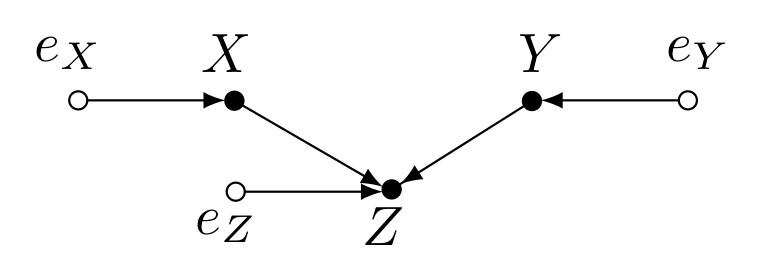
\includegraphics[width=1\textwidth,height=\textheight]{images/figures/mdag_bb5.png}

}

\subcaption{\label{fig-mdag_bb5}Collider or inmorality}

\end{minipage}%
%
\begin{minipage}{0.33\linewidth}

\centering{

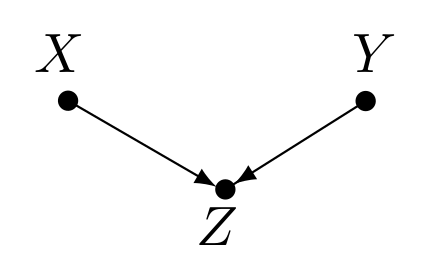
\includegraphics[width=0.55\textwidth,height=\textheight]{images/figures/sdag_bb5.png}

}

\subcaption{\label{fig-sdag_bb5}Collider or inmorality}

\end{minipage}%
%
\begin{minipage}{0.33\linewidth}

\centering{

\[
\begin{aligned}
  X & := f_{X}(e_{X}) \\
  Z & := f_{Z}(X,Y,e_{Z}) \\
  Y & := f_{Y}(e_{Y}) \\
  e_{X} & \perp\!\!\!\perp e_{Y} \\
  e_{X} & \perp\!\!\!\perp e_{Z} \\
  e_{Z} & \perp\!\!\!\perp e_{Y}
\end{aligned}
\]

}

\subcaption{\label{fig-scm_bb5}Collider or inmorality}

\end{minipage}%

\caption{\label{fig-dags_scms}The five fundamental building blocks of
DAGs. \textbf{Note:} left panels show the magnified representation,
middle panels show the standard representation, and the right panels
show their corresponding SCM form.}

\end{figure}%

The left panels of Figure~\ref{fig-dags_scms} illustrate the
\emph{magnified} representation. These graphs depict the
\emph{endogenous} variables \(V=\{X,Z,Y\}\) alongside the
\emph{exogenous} variables \(E=\{e_{X},e_{Z},e_{Y}\}\). Endogenous
variables are those whose causal mechanisms the investigator chooses to
model \citep{Neal_2020}. In contrast, exogenous variables represent
\emph{errors} or \emph{disturbances} arising from omitted factors that
the investigator chooses not to model explicitly
\citep[27,68]{Pearl_2009}. The graphs show endogenous variables as solid
black circles to signify that they are observed random variables, while
endogenous variables are depicted as open circles to signify their
unobserved (latent) nature. Lastly, the arrows in the graphs reflect the
expected direction of causal influences among these variables.

Often, DAGs omit the exogenous variables for simplicity, resulting in
the \emph{standard} representation. However, including exogenous
variables in a graph can be beneficial in some scenarios, as their
presence can reveal potential issues related to conditioning and
confounding \citep{Cinelli_et_al_2020}, concepts explored in
Section~\ref{sec-framework-flow}. The standard representation is
illustrated in the middle panels of Figure~\ref{fig-dags_scms}.

Lastly, the right panels of Figure~\ref{fig-dags_scms} depict the SCM
form of the fundamental building blocks. SCMs are formal mathematical
models defined by a set of endogenous variables \(V\), a set of
exogenous variables \(E\), and a set of functions
\(F=\{f_{X},f_{Z},f_{Y}\}\) \citep{Pearl_2009, Neal_2020}. These
functions, referred to as structural equations, specify each endogenous
variable as nonparametric functions of other variables. Moreover, SCMs
use the symbol `\(:=\)' to indicate the variables' asymmetrical causal
dependence and the symbol `\(\perp\!\!\!\perp\)' to represent
\emph{d-separation}, which roughly equates to the concept of variable
independence. The concepts of d-separation and causal (in)dependence are
explored in Section~\ref{sec-framework-flow}.

A careful examination of Figure~\ref{fig-dags_scms} highlights the
assumptions underlying these building blocks. Figures
\ref{fig-mdag_bb1}, \ref{fig-sdag_bb1}, and SCM \ref{fig-scm_bb1} depict
two unconnected nodes, representing a scenario where variables \(X\) and
\(Y\) are not causally related. Figures \ref{fig-mdag_bb2},
\ref{fig-sdag_bb2}, and SCM \ref{fig-scm_bb2} illustrate two connected
nodes, showing a scenario where a \emph{parent} node \(X\) exerts a
causal influence on a \emph{child} node \(Y\). Consequently, \(Y\) is
considered a \emph{descendant} of \(X\). Figures \ref{fig-mdag_bb3},
\ref{fig-sdag_bb3}, and SCM \ref{fig-scm_bb3} depict a \emph{chain} or
\emph{pipe}, where \(X\) influences \(Z\), and \(Z\) influences \(Y\).
In this configuration, \(X\) is a parent node of \(Z\), and \(Z\) is a
parent node of \(Y\). This creates a \emph{directed path} between \(X\)
and \(Y\). Consequently, \(X\) is an \emph{ancestor} of \(Y\), and \(Z\)
fully \emph{mediates} the relationship between the two. Figures
\ref{fig-mdag_bb4}, \ref{fig-sdag_bb4}, and SCM \ref{fig-scm_bb4}
illustrate a \emph{fork}, where variables \(X\) and \(Y\) are both
influenced by \(Z\). Here, \(Z\) is a parent node of \(X\) and \(Y\).
Finally, Figures \ref{fig-mdag_bb5}, \ref{fig-sdag_bb5}, SCM
\ref{fig-scm_bb5} depict a \emph{collider}, also known as
\emph{inmorality}, where variables \(X\) and \(Y\) are concurrent causes
of \(Z\). In this configuration, \(X\) and \(Y\) are not causally
related to each other but both influence \(Z\). Additionally, in all
SCMs, the errors are assumed to be mutually independent of each other
and of all other variables in the graph, as evidenced by the pairwise
relations \(e_{X} \perp\!\!\!\perp e_{Y}\),
\(e_{X} \perp\!\!\!\perp e_{Z}\), and \(e_{Z} \perp\!\!\!\perp e_{Y}\).

The motivating example in Section~\ref{sec-framework-structural} can
further illustrate how to use the five fundamental building blocks to
construct a system's causal structure. In this scenario, the
investigator aims to determine whether, \emph{on average}, there is a
difference in conceptual understanding of a topic \((Y_{i}=\{0,1\})\)
between two groups of students \((T_{i}=\{1,2\})\), described by the
estimand \(E[Y_{i}| T_{i}=1] - E[Y_{i}| T_{i}=2]\). However, unlike the
previous case, an experiment cannot be conducted, and the problem
suggests that the country to which a student belongs (\(X\)) may
influence both \(T\) and \(Y\). Such scenarios are plausible, especially
when the teaching methods depend on software or access to technology,
which may be limited in certain countries {(maybe an example with more
impact?)}. Figure~\ref{fig-example} illustrates the plausible causal
structure of the motivating example. A detailed examination of Figures
\ref{fig-mdag_example1}, \ref{fig-sdag_example1}, and SCM
\ref{fig-scm_example1} reveals the presence of at least four of the five
fundamental building blocks. The figures display multiple descendants,
as indicated by pairwise relations such as \(X \rightarrow T\),
\(X \rightarrow Y\), and \(T \rightarrow Y\). Additionally, the figures
features multiple pairs of unconnected nodes, evident from the relations
\(e_{T} \perp\!\!\!\perp e_{X}\), \(e_{T} \perp\!\!\!\perp e_{Y}\), and
\(e_{X} \perp\!\!\!\perp e_{Y}\). Finally, the figures illustrate the
fork \(X \rightarrow \{T,Y\}\), and two colliders with
\(\{X,e_{T}\} \rightarrow T\) and \(\{X,T,e_{Y}\} \rightarrow Y\).

\begin{figure}

\begin{minipage}{0.33\linewidth}

\centering{

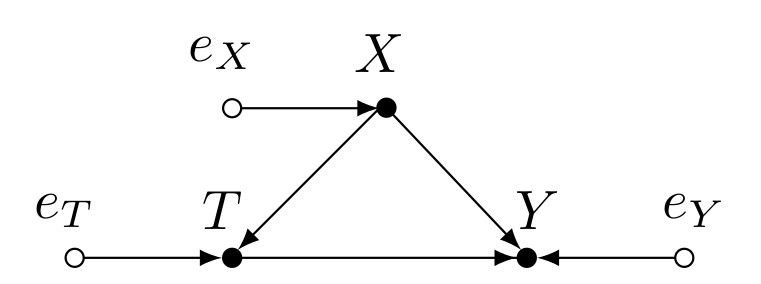
\includegraphics[width=1\textwidth,height=\textheight]{images/figures/mdag_example1.png}

}

\subcaption{\label{fig-mdag_example1}Magnified representation}

\end{minipage}%
%
\begin{minipage}{0.33\linewidth}

\centering{

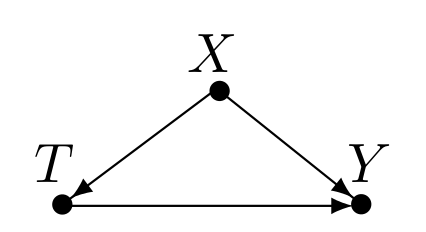
\includegraphics[width=0.55\textwidth,height=\textheight]{images/figures/sdag_example1.png}

}

\subcaption{\label{fig-sdag_example1}Standard representation}

\end{minipage}%
%
\begin{minipage}{0.33\linewidth}

\centering{

\[
\begin{aligned}
  X & := f_{X}(e_{X}) \\
  T & := f_{Z}(X,e_{T}) \\
  Y & := f_{Y}(T,X,e_{Y}) \\
  e_{T} & \perp\!\!\!\perp e_{X} \\
  e_{T} & \perp\!\!\!\perp e_{Y} \\
  e_{X} & \perp\!\!\!\perp e_{Y}
\end{aligned}
\]

}

\subcaption{\label{fig-scm_example1}Structural causal model}

\end{minipage}%

\caption{\label{fig-example}DAGs for a plausible causal structure in a
system.}

\end{figure}%

\subsection{The flow of association and causation in
graphs}\label{sec-framework-flow}

\begin{figure}

\centering{

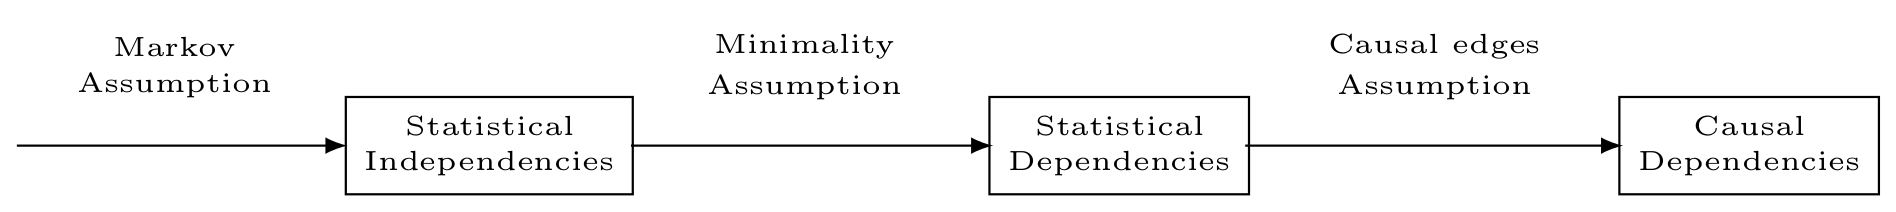
\includegraphics[width=0.8\textwidth,height=\textheight]{images/figures/ACflow.png}

}

\caption{\label{fig-ACflow}The flow of association and causation in
graphs. Extracted and slightly modified from \citet[31]{Neal_2020}}

\end{figure}%

\section{Theory}\label{sec-theory}

\subsection{A scientific model for the DCJ}\label{sec-theory-scientific}

\begin{figure}

\centering{

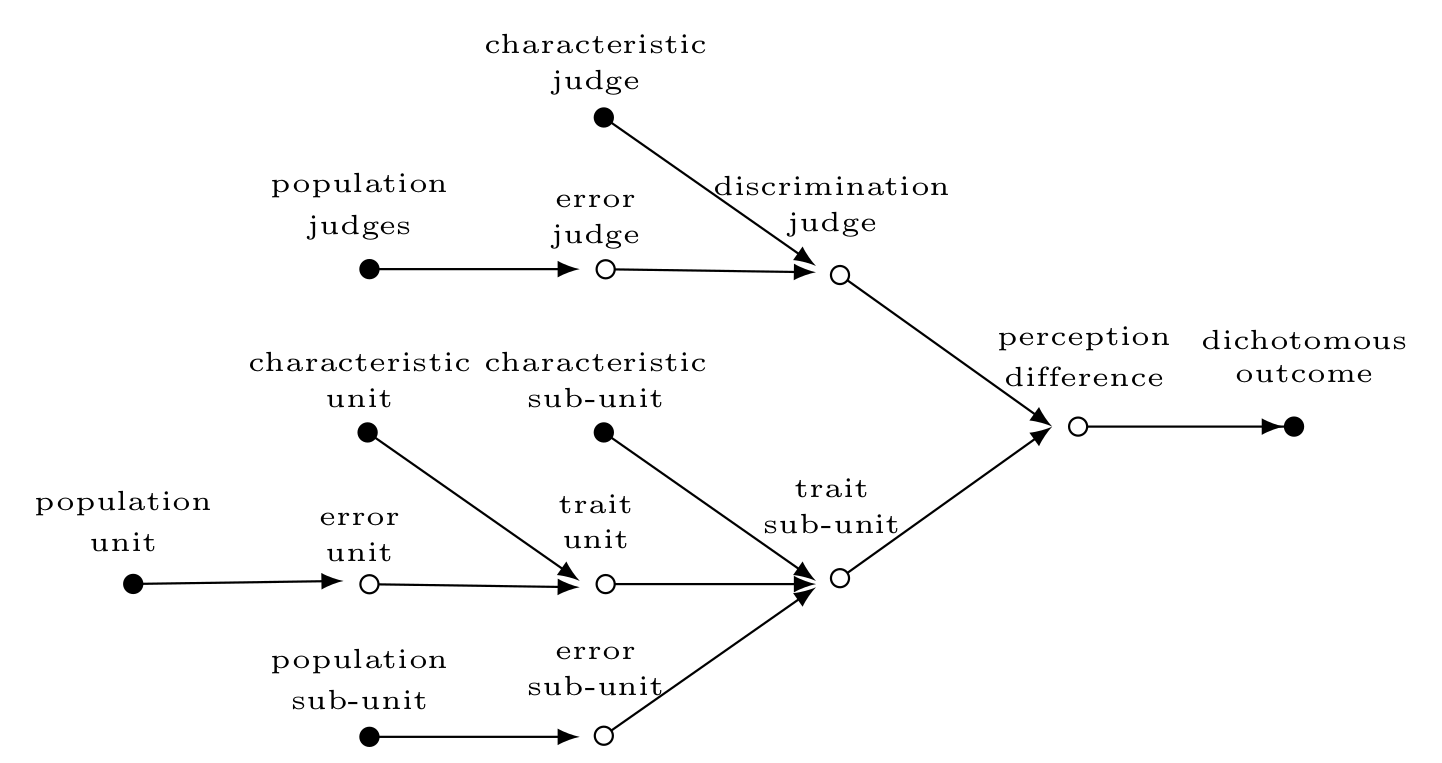
\includegraphics[width=0.8\textwidth,height=\textheight]{images/figures/SciModel_simp1.png}

}

\caption{\label{fig-SciModel_simp1}DCJ causal diagram, simplified
description}

\end{figure}%

\begin{figure}

\centering{

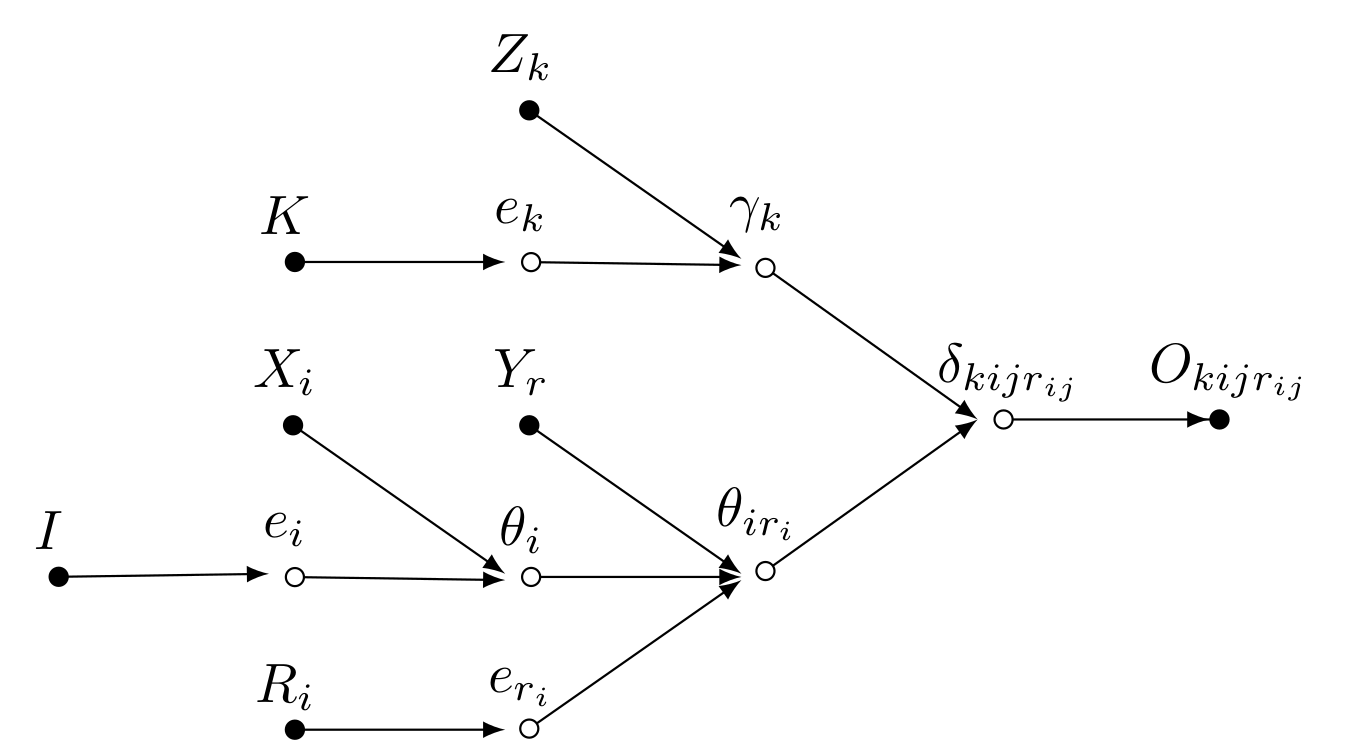
\includegraphics[width=0.7\textwidth,height=\textheight]{images/figures/SciModel_simp2.png}

}

\caption{\label{fig-SciModel_simp2}DCJ causal diagram, simplified
mathematical description}

\end{figure}%

\begin{figure}

\centering{

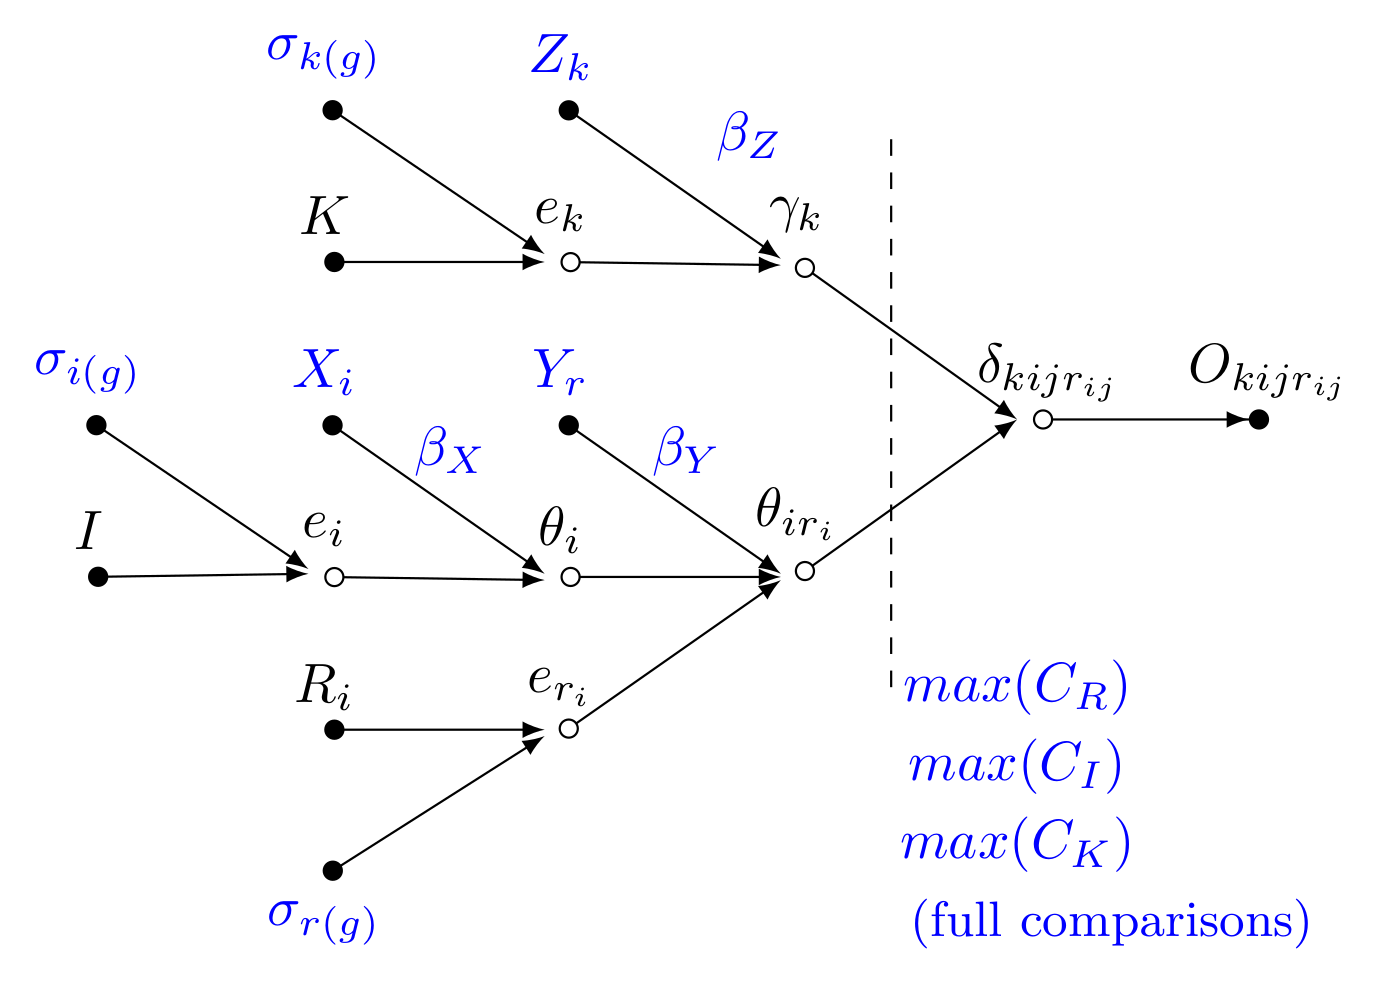
\includegraphics[width=0.7\textwidth,height=\textheight]{images/figures/SciModel_pop.png}

}

\caption{\label{fig-SciModel_pop}DCJ causal diagram, population
mathematical description}

\end{figure}%

\begin{figure}

\centering{

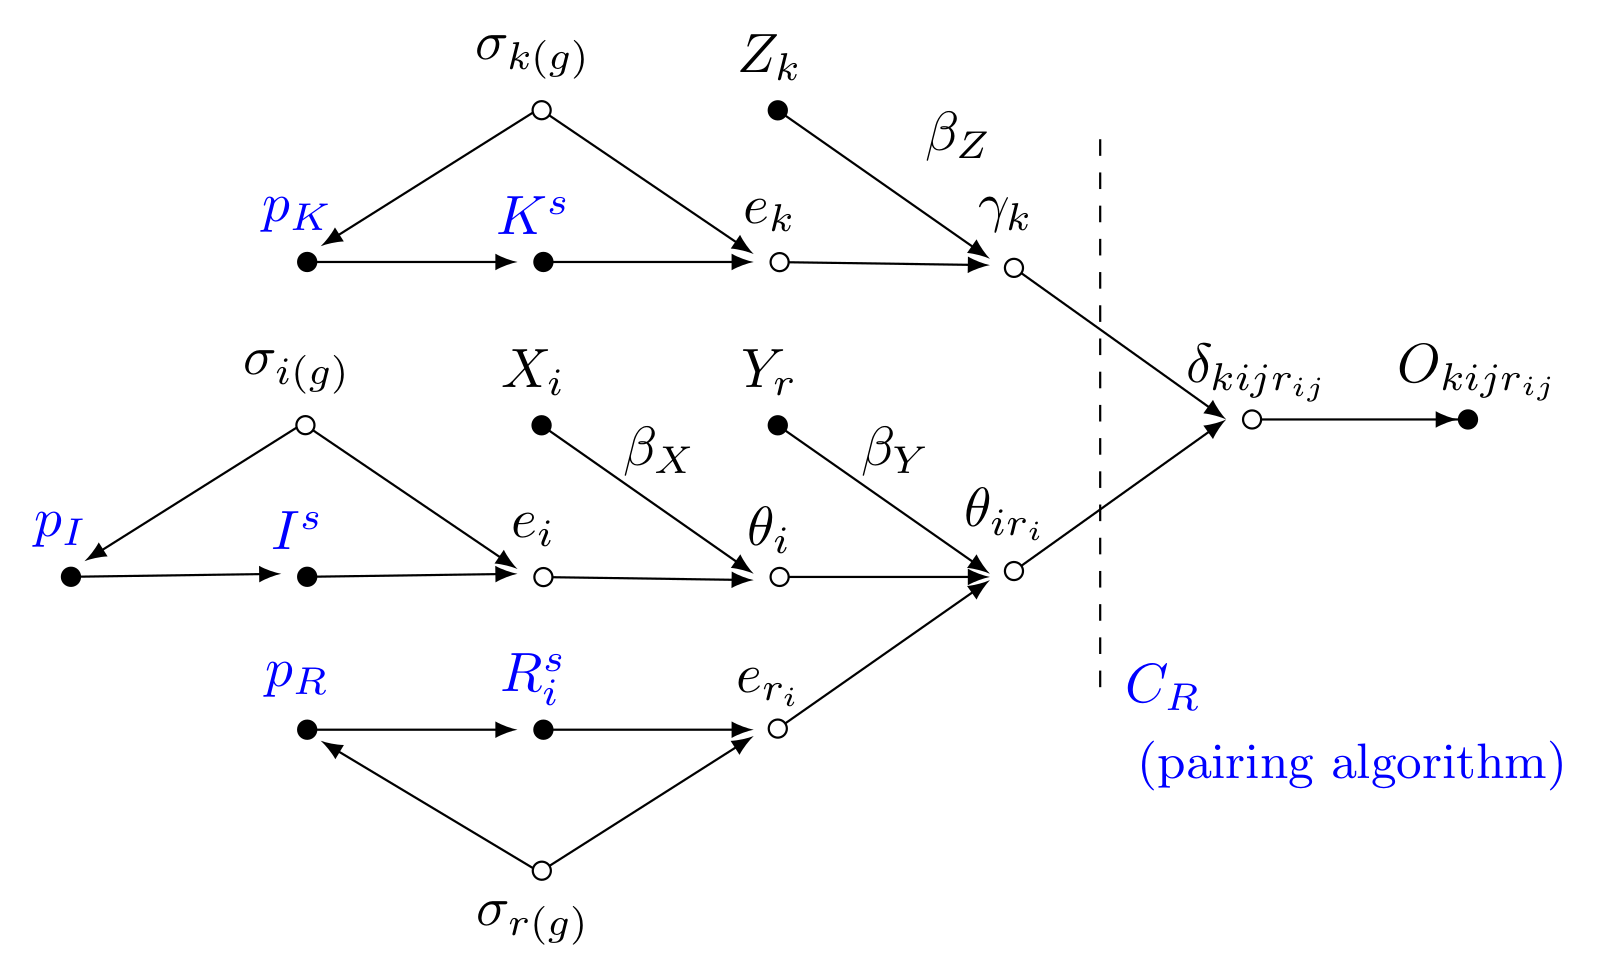
\includegraphics[width=0.8\textwidth,height=\textheight]{images/figures/SciModel_samp.png}

}

\caption{\label{fig-SciModel_samp}DCJ causal diagram, sample with
comparisons mathematical description}

\end{figure}%

\subsection{Probabilitics assumptions of the scientific
model}\label{sec-theory-probability}

\subsection{From the scientific to statistical
model}\label{sec-theory-statistics}

\subsection{Let's talk about Thurstone}\label{sec-theory-thurstone}

\section{Discussion}\label{sec-discuss}

\subsection{Findings}\label{sec-discuss-finding}

\subsection{Limitations and further
research}\label{sec-discuss-limitations}

\section{Conclusion}\label{sec-conclusion}

\newpage{}

\section*{Declarations}\label{declarations}
\addcontentsline{toc}{section}{Declarations}

\textbf{Funding:} The project was founded through the Research Fund of
the University of Antwerp (BOF).

\textbf{Financial interests:} The authors have no relevant financial
interest to disclose.

\textbf{Non-financial interests:} Author XX serve on advisory broad of
Company Y but receives no compensation this role.

\textbf{Ethics approval:} The University of Antwerp Research Ethics
Committee has confirmed that no ethical approval is required.

\textbf{Consent to participate:} Not applicable

\textbf{Consent for publication:} All authors have read and agreed to
the published version of the manuscript.

\textbf{Availability of data and materials:} No data was utilized in
this study.

\textbf{Code availability:} All the code utilized in this research is
available in the digital document located at:
\url{https://jriveraespejo.github.io/paper2_manuscript/}.

\textbf{Authors' contributions:} \emph{Conceptualization:} S.G., S.DM.,
T.vD., and J.M.R.E; \emph{Methodology:} S.DM., T.vD., and J.M.R.E;
\emph{Software:} J.M.R.E.; \emph{Validation:} J.M.R.E.; \emph{Formal
Analysis:} J.M.R.E.; \emph{Investigation:} J.M.R.E; \emph{Resources:}
S.G., S.DM., and T.vD.; \emph{Data curation:} J.M.R.E.; \emph{Writing -
original draft:} J.M.R.E.; \emph{Writing - review \& editing:} S.G.,
S.DM., and T.vD.; \emph{Visualization:} J.M.R.E.; \emph{Supervision:}
S.G. and S.DM.; \emph{Project administration:} S.G. and S.DM.;
\emph{Funding acquisition:} S.G. and S.DM.

\newpage{}

\section{Appendix}\label{sec-appendix}

\subsection{Why do we need to estimate judges'
abilities?}\label{sec-appA}

\subsection{Latent variables as a mean of imputation}\label{sec-appB}

\subsection{Other comparative scenarios}\label{sec-appC}

\newpage{}

\subsection*{References}\label{references}
\addcontentsline{toc}{subsection}{References}

\renewcommand{\bibsection}{}
\bibliography{references.bib}





\end{document}
